\documentclass{article}
\usepackage{ijcai13}
\usepackage{times}
\usepackage{latexsym} 

%\documentclass[letterpaper]{article}
%\usepackage{aaai}
%\usepackage{times}
%\usepackage{helvet}
%\usepackage{courier}
\usepackage{algorithm2e}
%\frenchspacing

\usepackage{graphicx}

\title{Leveraging Collaboration: 
A Methodology for the Design of Social Problem-Solving Systems}

\begin{document}

\maketitle

\begin{abstract}
Social collaboration has been shown to facilitate problem-solving activity in diverse sets of environments. 
Nevertheless, if not well designed, social and human computation systems may achieve results 
only similar to those of a single human subject performing a task. 
This scenario reflects a need for better understanding of the performance 
issues of human problem-solving social networks. 
Firstly, we propose a model for simulating social problem-solving. 
We then carry out several simulations with artificial agents  
supported by results of experiments carried out with human subjects, 
in order to analyse which parameters influence the performance of collaborative problem-solving social networks. 
We analyse the strategies humans follow when solving a problem, 
comparing them with alternative ones, and 
identify the consequences of the employed strategies 
in the collective performance of the social network. 
Our results also indicate that copying and guessing are beneficial to the 
performance of the social networks. 
We then propose mechanisms that can improve 
collaborative problem-solving.
Finally, we show that our results lead to a methodology for the design  
of efficient problem-solving systems that can be applied 
to several kinds of collaborative social systems. 

\end{abstract}

\section{Introduction}

%--Contextualização geral
For years multi-agent systems have been used to research cooperation as a tool for problem-solving. %cite Malone
Recently, however, there has been an increasing interest in the study of human beings as problem-solving agents. Several experiments have been conducted in which subjects are connected in a network with the goal of collectively solving a specific problem, and those have helped shed some light on the way humans interact to solve problems as well as on the dynamics of working groups~\cite{woolley:evidencecollective}.

%--O problema, por que ele é importante
However, although those studies can provide us with observations and hypotheses, there is still a difficulty in finding ways to explain the observed collective, human behaviour. In order to better employ human abilities to problem-solving, we need a method of studying that behaviour and its consequences.

Human beings are known to be able to easily perform tasks which are still generally difficult for computers, such as natural language processing and image recognition.
%--
However, it would be useful to apply human social computation to more straightforward computer problems with precise definitions and algorithms, but which are still computationally intensive.
%--
The different abilities of computers and humans suggest that the latter might provide a new approach to problems that might be more effective than current techniques employed by computers. That notion has been successfully applied, for example, in one of the most significant problems in the field of bioinformatics: protein structure prediction (PSP). A software that presents the problem to humans as an online computer game, called \emph{Foldit}~\cite{cooper:foldit}, has produced significant results in the research of PSP, which is usually approached as an optimization problem requiring extensive computational power. Such results have been attributed to human visual problem-solving and decision-making abilities, as well as social collaboration~\cite{cooper:foldit}. However, we still don't know the limits of human abilities in problem-solving and how they compare to more traditional computational techniques.

In order to take full advantage of human problem-solving strategies, we must learn their limitations. Humans tend to be less efficient than computers in mathematical computations, are subject to a series of physical and psychological conditions that might affect their performance, and do not always act rationally. Those are all factors that might come in the way of the problem-solving process, but by understanding their consequences we can find ways to sidestep them or even use them in our favour.

%--Como nós vamos resolver
In this paper, we use a multi-agent based simulation to complement %change?
the study of human computation, as a way of explaining the strategies used by humans when solving problems and understanding their consequences in a cooperative environment. The degree of control that simulations provide us over the behaviour of the agents allows us to better understand possible reasons for the actions and behaviours displayed by human agents.

Through this system, it becomes possible to draw new conclusions from past observations of human behaviour. The model can be used, for example, to preview the results that changes in the infrastructure of a social computation system will have on its performance before actually performing the experiments with humans. Another possibility is to use the results obtained by the simulation of past experiments to plan the configuration of a new system of social computing.

\section{Background}

Human and social computing are relatively new areas of research with a diversified, interdisciplinary root that mixes social sciences, artificial intelligence, game theory and network science, among others. %cite ?, Kleinberg
Only recently studies on the potential of human social networks for solving problems are gaining some popularity. %cite Malone, Kearns
Those have provided insights into, among other things, the impact of network structure in the collaboration process and the factors that lead neighbours' proposed solutions to be copied by individuals.

The origin of human computation as we know it today can be traced back to the work of~\cite{vonahm:gwap}, which identified the possibility of using entertainment as an incentive to participation of human subjects, applying it in games in which the participants are actually performing a computation. That is an idea that also appears in the Foldit game~\cite{cooper:foldit}.

The series of experiments summarized in~\cite{kearns:experim} are among the first to try to take advantage of collective problem-solving abilities to solve classical computer problems. The experiments are mostly based on the concept of coordination: subjects have individual incentives that are expected to drive them to cooperate with one another and lead them toward the collective goal~\cite{nowak:evolutioncooperation}.

Other initiatives have appeared, such as the ones by~\cite{farenzena:collabem} and~\cite{mason:collablearnet}, which take a different approach by having subjects trying to solve the collective problem individually, with the possibility of exchanging solutions between neighbours. Those have resulted in interesting conclusions on human behaviour when the possibility of copying peers is available. Our experiments follow this line of research.

The experiments conducted by~\cite{farenzena:collabem} had human beings trying to solve constraint satisfaction problems, namely Boolean Satisfiability (SAT)~\cite{cook:complexitytheoremproving} and the popular \emph{Sudoku} game~\cite{weber:satsudoku}, with individuals connected through the network being able to exchange partial solutions of the problem in question.
In that study a specific pattern of behaviour was observed which suggests that humans didn't evaluate the solutions proposed by their neighbours, instead choosing to copy the solutions which were displayed closer in the system's interface.
That behaviour is referred to as an evidence of conformism in human subjects. On the other hand,~\cite{mason:collablearnet} seem to suggest that their subjects did evaluate the available solutions, although %Unfortunately?
an in-depth analysis of that fact was not reported. That might mean that multiple factors might influence the behaviour of human agents. We analyse possible reasons in section~\ref{sec:discuss}.

\section{Contribution}

%--Principais resultados
We developed a novel method for artificial social problem-solving that can be used to simulate the behaviour observed in humans in collective problem-solving systems. This model is described on section~\ref{sec:model}.

The methodology was then applied to build a multi-agent system that simulates the experiments of~\cite{farenzena:collabem}, using the model of human behaviour proposed by them. We describe how we adapted that environment and the behaviour of its subjects to our system in section~\ref{sec:setup}. We limited our experiments to the Sudoku problem, which is more attractive and accessible to human beings while being NP-complete and equivalent to SAT. However, the results obtained can be generalized to different problems.

In the experiments performed by~\cite{farenzena:collabem}, it was verified that the human subjects didn't evaluate their neighbours' solutions, instead choosing an arbitrary solution based on position in the interface. We simulated that behaviour in our agents and compared that strategy with an alternative, artificial strategy, and reached the conclusion that the human strategy is detrimental to the problem-solving process. A network of agents that evaluated the solutions proposed to them performed consistently better, even though the evaluation function employed wasn't one that accurately represented the solution's worth. That way, we verify that even a naive evaluation tactic surpasses choosing an arbitrary neighbour to copy. A more detailed analysis is provided in sections~\ref{sec:results} and~\ref{sec:discuss}. In the same section, we analyse the impact that copying and guessing have on the process of solving the problem. After obtaining those results, we are able to propose a set of guidelines for the design of social problem-solving systems that might address those issues and improve the performance of human computing.

\section{A Novel Method for %Artificial?
Social Problem Solving}
\label{sec:model}

A number of multi-agent methodologies that employ information flow through agents have been studied before. For instance, the {\em Memetic Networks} model proposed by~\cite{araujo:memenet} draws inspiration from the phenomenon of {\em Cultural Evolution} discussed by Dawkins in~\cite{dawkins:selfishgene} and has a network of agents sharing, copying and incrementing units of information in a similar way that nature, according to Dawkins, deals with {\em Memes}~\cite{dawkins:selfishgene}. Nevertheless, some aspects of social behaviour of great significance to social computing cannot be properly analysed through this methodologies. One example is the conformist behaviour studied in~\cite{cefferson:conformists} and~\cite{farenzena:collabem}. The proper study of these aspects demands a novel method for artificial collaborative problem solving.

We propose a method for solving computational problems by means of a network of agents endowed with social behaviour. Our algorithm is composed of an ordered set of $N$ agents, each encoding a partial solution to the problem, and a binary $N \times N$ matrix representing possible connections between agents. Additionally, our algorithm is composed of two stages, namely the {\em communication phase} and the {\em reasoning phase}.

\begin{algorithm}
 \SetAlgoLined
 Initialize N agents, each encoding a partial solution to the problem\;
 \While{termination condition not met}
 {
 	\For{i = 1 to N}
 	{
 		\For{j = 1 to N}
 		{
 			\If{j is connected to i}
 			{
 				$A_{i}$ = $i_{th}$ agent\;
 				$A_{j}$ = $j_{th}$ agent\;
 				Add $A_{j}$'s solution to the collection of messages received by $A_{i}$\; %A.messages.add(j.solution)\;
 			}
 		}
 	}
 	\For{i = 1 to N} 
 	{
 		\CommentSty{ //Communication Phase }\;
 		$A_{i}$ = $i_{th}$ agent\;
 		selectedMessage = select($A_{i}$.messages)\;
 		
 		\If{random(0,1) $<$ copyRate}
 		{
 			$A_{i}$.solution = selectedMessage\;
 		}
 	}
 	\For{i = 1 to N}
 	{
 		\CommentSty{ //Reasoning Phase }\;
 		$A_{i}$ = $i_{th}$ agent\;
 		Add local changes to $A_{i}$'s solution%$A_{i}$.solution = addLocalChanges($A_{i}$.solution)\;
 	}
 }
 \caption{Algorithm for the proposed model, encompassing the communication and reasoning phases}
\end{algorithm}

\begin{itemize}
\item
Communication phase: In the communication phase, messages are passed from agent to agent through the network connections. Agents are thus presented with a multiplicity of messages. There is a particular probability associated with the behaviour of agents choosing to copy one of these solutions in contrast to keeping their current solutions. We call this probability the \emph{copy rate}. When an agent chooses to copy, it is then supposed to select for copying a single one of its received messages. This is done by means of a particular message-selecting strategy.

\item
Reasoning phase: In the reasoning phase, agents are supposed to add local changes to the messages copied in the previous stage. This is done by means of a heuristic or an exact method.
\end{itemize}

\section{Experimental Setup}
\label{sec:setup}

In order to validate our method as a social problem-solving model, we have modelled the real-world collaborative Sudoku solving environment studied in~\cite{farenzena:collabem} through our method and tested it over a set of Sudoku instances.

\subsection{Communication Phase}

The experiments conducted by~\cite{farenzena:collabem} point out a series of observations about the dynamics of cooperation in problem solving with human beings. For instance, the authors' analysis has shown that human subjects are more likely to engage in the behaviour of copying the most readily available solutions on the graphic interface than in that of evaluating the available solutions and choosing the best according to some criterion. We have modelled two message-selecting strategies to employ in the communication phase, where one attempts to evaluate the solutions and choose the best one and the other mimics the human behaviour of selecting the first solutions with greater probability.

Although employed by us in the context of the Sudoku problem, these strategies can be generalized to apply to different problems. It was verified in~\cite{farenzena:collabem} that the human behaviour of copying arbitrary solutions was not strictly dependent on the problem, since similar results were obtained for both SAT and Sudoku.

\subsubsection{{\em Most Filled} strategy}

This strategy employs the intuitive strategy of selecting the most complete message for copying. For example, in the SAT problem the most complete solution could be the one with the most clauses that evaluate to \emph{true}. In the specific case of Sudoku solving, this strategy selects the most filled Sudoku partial solution. Put in other words, it selects the Sudoku partial solution with the least number of blank cells. This is an attempt at a strategy that evaluates the messages that arrive to the agent and chooses the best solution. It is important to notice, however, that it doesn't guarantee that the chosen solution is actually better, since it might contain errors. In the case of Sudoku, a cell might be marked with wrong value.

\subsubsection{{\em First Positions} strategy}

We know that, in some settings of collaborative problem-solving, human subjects are likely to copy the first (from left to right) solutions on the graphic interface~\cite{farenzena:collabem}. The authors have provided us with a mathematical model of this behaviour, stated as $\langle X(k)\rangle = (1-p)^{k-1}p$, where the parameter $p$ is fixed as $p = 0.5479$ and $\langle X(k)\rangle$ denotes the probability of an agent copying the $k_{th}$ neighbour solution.

We inserted this behaviour into our model by firstly generating a random ordering of neighbours for each agent in order to compose a simulated graphic interface. As a result, each agent visualizes some neighbours before or after others. Secondly, we translated the above mathematical model into a message-selecting strategy in which the solution selected by an agent is the $k_{th}$ with probability $\langle X(k)\rangle$.

\subsection{Reasoning Phase}

The techniques employed by the agents to advance the solution individually should be chosen according to the problem in question. In the case of Sudoku, solving techniques are abundant in literature. %Sudoku strategy literature?
These techniques are based on the reasoning usually employed by humans to solve Sudoku puzzles. Davis~\cite{davis:mathsudoku} discusses a collection of these techniques, of which the {\em Naked Singles} rule, the {\em Hidden Singles} rule and the {\em Naked Twins} rule are some examples. These techniques intend to, given a partial Sudoku solution, generate a set of {\em movements} which can be used to mark cells of this Sudoku puzzle. We implemented five of these rules, modelling each one of them as a function that maps a Sudoku partial solution to a set of movements. These functions can be used in the reasoning phase to add local changes to the Sudoku message received in the communication phase.

The rules implemented were the {\em Unique Missing Candidate} rule, the {\em Naked Singles} rule, the {\em Hidden Singles} rule, the {\em Two out of Three} rule and the {\em Naked Twins} rule, all of which (with the exception of the {\em Two out of Three} rule) are discussed in~\cite{davis:mathsudoku}. In our modelling, each agent knows a particular quantity of rules, this quantity determining the agent's {\em level}. For instance, an agent of level 3 knows three out of the five rules. Agents of level 0 know no rules and therefore can only guess and copy. That way, we model a wide range of skills that might be found in human agents. Our tests were all conducted with a heterogeneous population of agents of different levels. We detail below the 'two out of three' rule. For details on the other four rules, see~\cite{davis:mathsudoku}.

\subsubsection{Two out of Three Rule}

This rule applies to groups of three contiguous $3 \times 3$ blocks. It aims to find a value $v$ such that $v$ is present in two of the three $3 \times 3$ blocks encompassed by the group, but missing on the third. It proceeds by enumerating all the candidate cells - namely the empty cells - on this block, and then, by eliminating from this set all the cells that belong to the rows or columns in which $v$ is placed on the other two blocks. If the resulting set has cardinality $1$, the rule has successfully found a cell to mark.

%--Keep?
\subsection{Copying Solutions}

In the study conducted by~\cite{farenzena:collabem}, subjects were invited to solve Sudoku puzzles and share them with other subjects with whom they were connected through a network topology. At any time, a player could copy solutions from one of his or her neighbours. The authors' analysis has shown that there is a different copy frequency associated with each topology. For instance, the scale free topology with $\gamma = 1.65$ resulted in a copy frequency of $87 \%$, while the fully connected topology resulted in a copy frequency of $42 \%$.

We incorporated this copying frequency into our modelling, recreating the scenario of the experiments conducted by~\cite{farenzena:collabem} by setting this parameter accordingly to the topologies we used.
%--

\subsection{Guessing and Backtracking}

We have consistent evidence that trial-and-error is a part of the Sudoku solving experience. The need for trial-and-error in Sudoku puzzles is not a falsifiable conclusion, but a mathematical fact~\cite{davis:mathsudoku}. Some puzzles are only solvable by the means of a backtracking procedure.

In our modelling, we associate each agent with a numerical parameter determining the probability this agent has to guess when incapable of applying a typical Sudoku solving strategy. We call this parameter the \emph{guess rate}.

Automatic Sudoku solvers employing a backtracking algorithm are easily programmed and very time-efficient. On the other hand, the space complexity of these algorithms is a barrier to most human solvers, who need to write down tons of observations in order to employ a backtracking strategy. With this in mind, we propose in our modelling a different kind of backtracking, intended to be more similar to the way human beings employ error correction in Sudoku solving in a collaborative environment such as the one analysed in~\cite{farenzena:collabem}, which we refer to as \emph{social backtracking}. In it, when faced with one or more conflicts in its own solution, an agent copies a solution from one of its neighbours. In our modelling, this is done by raising the copy rate of this particular agent to $100 \%$.

\subsection{Network Topology}

We modelled our agent networks through the network topologies employed by~\cite{farenzena:collabem} in their tests with human social networks. The topologies used were the {\em fully connected} topology, the {\em scale-free} topology~\cite{barabasi:linked}, the {\em 2-Ring} topology and the {\em 3-Ring} topology~\cite{newman:newtorks}.

\section{Experiments and Results}
\label{sec:results}

We tested the simulated Sudoku environment using an heterogeneous, uniform agent distribution in which every agent level (0 to 5) %explain; table?
had an equal representation in the population. We performed experiments with varying message selecting strategies, network topologies and values for the parameters of copy rate and guess rate.

\begin{figure}
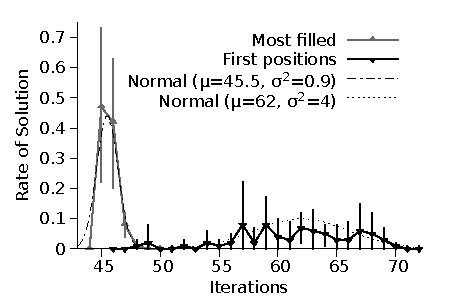
\includegraphics[scale=1]{ijcai_sudoku/ring}
\caption{The graph presents the average results for the 3-ring topology, showing the proportion of agents to obtain the correct solution on each round for both the \emph{Most Filled} and \emph{First Positions} strategies. The lines for both strategies can be fitted to normal distributions with different values for mean and variance.}
\label{fig:ring_gauss}
\end{figure}

\begin{figure}
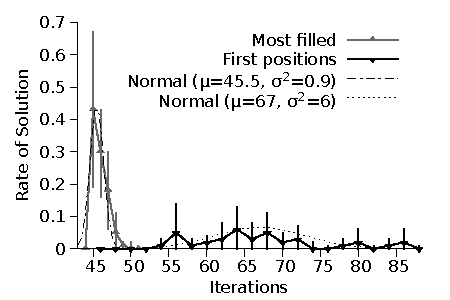
\includegraphics[scale=1]{ijcai_sudoku/sf}
\caption{The graph presents the average results for the scale-free topology, showing the proportion of agents to obtain the correct solution on each round for both the \emph{Most Filled} and \emph{First Positions} strategies. The lines for both strategies can be fitted to normal distributions with different values for mean and variance.}
\label{fig:sf_gauss}
\end{figure}

\begin{figure}
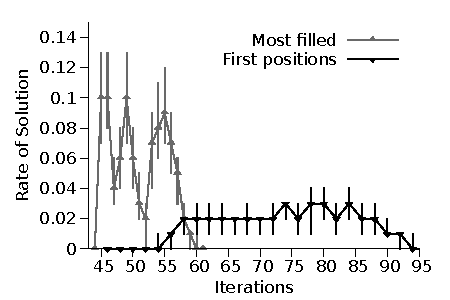
\includegraphics[scale=1]{ijcai_sudoku/geral}
\caption{The graph presents the average results for all topologies and instances, showing the proportion of agents to obtain the correct solution on each round for both the \emph{Most Filled} and \emph{First Positions} strategies. The lines for both strategies can be fitted to normal distributions with different values for mean and variance.}
\label{fig:global_gauss}
\end{figure}

\subsection{Comparison of Copying Strategies}

%--Descrever experimentos
We have run experiments with four different topologies, previously enumerated in section~\ref{sec:setup}, for seven different problem instances, and obtained similar results in each. We used fixed values of copy rate and guess rate in all runs. Each experiment ran for 100 rounds composed of a communication phase and a reasoning phase. For each combination of topology and instance we ran once using the \emph{Most Filled} strategy and again using the \emph{First Positions} strategy, with the goal of comparing their performance. Our hypothesis was that the \emph{Most Filled} strategy would perform better, a result which would confirm our belief that problem-solving social networks respond positively to the employment of evaluation functions.

%--Descrever resultados
We have observed in our experiments that the progress of the solution, represented by the number of agents that solve the problem in a given round, follows a normal distribution. During the first rounds no agents have found the solution. Then the first few agents solve the problem. The round in which that happens varies according to the particular instance of the problem. From that point onwards the final solution starts spreading throughout the network. As more agents obtain the complete solution, it becomes more likely that further agents will copy that solution from their neighbour, which complies with a conformist behaviour, as observed in~\cite{farenzena:collabem}. 
The number of agents with complete solutions increases in the following rounds, until it reaches a point where the few remaining agents take longer to obtain the solution due to factors such as being less skilled solvers or being in unfavourable positions in the topology.

The solution progress for the \emph{Most Filled} and \emph{First Positions} strategies can be described as normal distributions of different mean and variance. In the experiments, the mean indicates how soon the correct solution was found, and the variance how long the final solution took to spread throughout the network. The exact values for those parameters vary according to factors such as topology and problem instance, but they follow a particular pattern: in all cases, the \emph{Most Filled} strategy has lower mean - indicating the solution is found sooner - and lower variance - meaning it spreads faster. 
We have chosen the scale-free and 3-ring topologies as representative examples, and plotted the average of the results for the same instance of the problem for each topology in Fig.~\ref{fig:ring_gauss} and~\ref{fig:sf_gauss}, respectively. Each graph shows the average of the percentage of agents that find the correct solution in each round for the two strategies, with normal curves plotted over the values evidencing the behaviour described above. One notes that the results fluctuate more for the second strategy, which is explained by its nearly random method of choosing solutions to copy.

Fig.~\ref{fig:global_gauss} depicts the average for all experiments, encompassing every topology and instance. In this graph, the presence of the normal behaviour in the distribution is less clear, because it combines several different instances and topologies. Nevertheless, its effects can still be seen. The \emph{Most Filled} strategy displays different residual peaks from particular instances, while the line for the \emph{First Positions} strategy starts flattening with the accumulation of several distributions from the individual experiments. More importantly, 
Fig.~\ref{fig:global_gauss} shows that the results of Fig.~\ref{fig:ring_gauss} and~\ref{fig:sf_gauss} can be generalized: in average, for every topology and instance, the network converged to the correct solution between rounds 44 and 60 with the \emph{Most Filled} strategy, and between rounds 54 and 94 with the \emph{First Positions} strategy, showing that for the \emph{Most Filled} strategy the solution is found earlier and spreads faster.

\begin{figure}
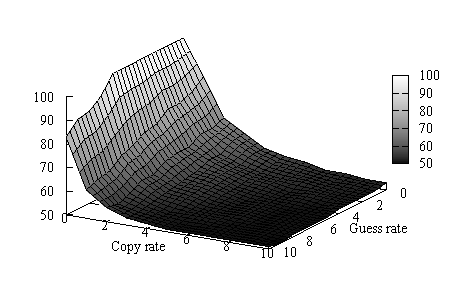
\includegraphics[scale=1]{ijcai_sudoku/fill_iter}
\caption{The graph shows the average number of iterations needed for all agents to obtain the correct solution, for a given value of copy rate and guess rate when using the \emph{Most Filled} strategy.
}
\label{fig:fill_iter}
\end{figure}

\begin{figure}
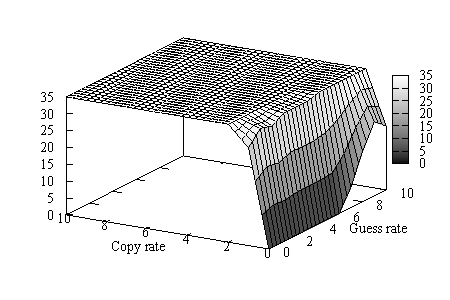
\includegraphics[scale=1]{ijcai_sudoku/fill_suc}
\caption{The graph shows the number of experiments in which all agents obtained the correct solution, for a given value of copy rate and guess rate when using the \emph{Most Filled} strategy.
}
\label{fig:fill_suc}
\end{figure}

\begin{figure}
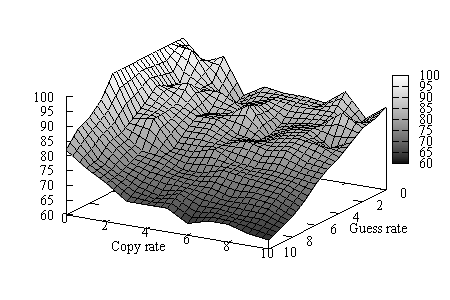
\includegraphics[scale=1]{ijcai_sudoku/first_iter}
\caption{The graph shows the average number of iterations needed for all agents to obtain the correct solution, for a given value of copy rate and guess rate when using the \emph{First Positions} strategy.
}
\label{fig:first_iter}
\end{figure}

\begin{figure}
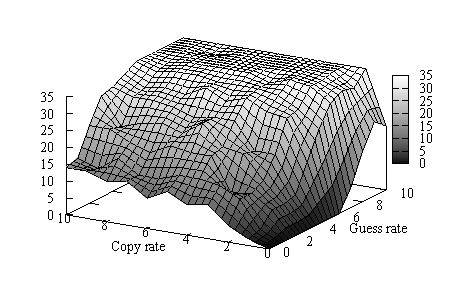
\includegraphics[scale=1]{ijcai_sudoku/first_suc}
\caption{The graph shows the number of experiments in which all agents obtained the correct solution, for a given value of copy rate and guess rate when using the \emph{First Positions} strategy.
}
\label{fig:first_suc}
\end{figure}

\subsection{Variation in Copy Rate and Guess Rate}

%--Descrever experimentos
The authors of~\cite{farenzena:collabem} have stated that, in their settings, {\em "cooperation works because agents can copy each other"}. Basing ourselves in that statement, we adopted the hypothesis that a higher copy rate would improve performance of the network. On the other hand, regarding the process of guessing we took the opposite standing, that it would decrease performance. We based that hypothesis on the notion that, when an agent makes a guess, it has a high chance of filling a cell with the wrong value. Once that happens, that grid will assuredly be unable to lead to the right solution until the agent copies a grid without errors from one of its neighbours. Therefore, we hypothesised that if an agent cannot make a logical move using its level of Sudoku-solving skills, it is better for it to wait for its neighbours to improve the solution and copy from them, instead of risking making an incorrect move.

In order to test our hypotheses, we repeated our experiments for the same four topologies, this time varying the copy rate and guess rate between $0\%$ and $100\%$ each. From our results for each topology, we plotted two surfaces for each strategy. The first shows the average number of iterations needed for the network to converge to the correct solution, and the second the number of experiments in which every agent obtained the correct solution in the limit of 100 rounds.

%--Descrever resultados
Fig.~\ref{fig:fill_iter} and Fig.~\ref{fig:first_iter} show the average number of rounds needed for the network to converge to the correct solution for the \emph{Most Filled} and \emph{First Positions} strategy, respectively. They both show a maximum in (copy rate: 0, guess rate: 0) and a minimum in (copy rate: 100, guess rate: 100), with greater copy rate and guess rate decreasing the number of rounds needed for the agents to solve the problem.

The results also differ depending on the copying strategy employed in the communication phase. Fig.~\ref{fig:fill_iter} shows that, using the \emph{Most Filled} strategy, as copying increases the number of rounds needed for all agents to have the correct solution decreases sharply until it stabilizes in a roughly optimal level. Similarly, in Fig.~\ref{fig:fill_suc} the number of experiments in which every agent obtains the correct solution rises fast as copying increases. Meanwhile, the benefits of guessing are much less pronounced. On the other hand, when the agents don't evaluate the neighbours' solutions, as can be seen in Fig.~\ref{fig:first_iter} and Fig.~\ref{fig:first_suc}, their contributions don't differ as much.

\section{Discussion}
\label{sec:discuss}

\subsection{A Novel Method For Simulating Human Problem-Solving Networks}

We have proposed a model to simulate human behaviour in a problem-solving social network. Through it, one can simulate previous experiments performed on humans by modelling the observed behaviour as the reasoning and communication phases. That way, one can examine the consequences of that behaviour without having to enlist human subjects, which is usually expensive and time-consuming~\cite{?}. Moreover this model can be used as a guide of what to look for in the data collected by the experiments, in which the strategies employed by the subjects to solve the problem individually are mapped into the reasoning phase and the strategy employed to pick a neighbour to copy, into the communication phase.

We have applied the model into one such human computing experiment and reached particular conclusions about the methods employed on it by humans. Since the same behaviour was observed for different problems, we can expect these results to be generalized to a certain class of problems and systems with specific characteristics. We provide further analysis below.

\subsection{Evaluating Neighbours' Solutions is Advantageous}

Our comparison between the \emph{Most Filled} and \emph{First Positions} strategies has shown that evaluating the neighbours' proposed solutions indeed brings significantly better results, despite the fact that humans seemingly avoid that strategy~\cite{farenzena:collabem}. In all topologies, choosing the solution with the largest number of filled cells not only allows agents to solve the instance earlier, but also causes the network to converge faster to the correct solution. That is, once one individual has found the correct solution, that solution spreads faster through the network if the other agents are evaluating the solutions that reach them instead of copying an arbitrary one.

Although choosing a solution based on its position instead of content is provably inefficient, this behaviour has been observed in human networks~\cite{farenzena:collabem}. Perhaps this can be explained 
by humans finding it difficult to evaluate Sudoku partial solutions. 
Although we have used the number of filled cells as a solution evaluation function, that is not guaranteed to accurately measure which solution is best, since individuals might fill in cells with the wrong value. That hypothesis is supported by the experiments of~\cite{mason:collablearnet}, which used optimization of a bi-dimensional function as the problem being solved. This problem has a straightforward and accurate method of determining the fitness of a solution, which is simply the value of the given function for the proposed coordinates. In their experiments, the subjects seemingly did effectively evaluate the proposed solutions, giving preference to the ones that were better evaluated. The difference in behaviour between the two experiments might be because in the latter the fitness of a certain solution was obvious to the agent, while in the former it's not as easy to pick the best solution out of the available ones.

Our experiments, however, have shown that although completeness is not necessarily an accurate measurement of quality, it was good enough to lead the network to the right solution.
Those results might extend to other constraint satisfaction problems that don't have an accurate method of evaluation. Therefore, it is not necessary for the problem addressed to have an exact evaluation function to compare different possible solutions. An imperfect evaluation is good enough to be employed in a problem-solving social network.

\subsection{Copying and Guessing are Beneficial to the Algorithm's Performance}

Regarding our hypothesis that a higher copy rate would be beneficial, our experiments indicate that in the topologies tested the copy rate indeed has a decisive role in enhancing the network's performance. To our surprise, however, they also indicate that guessing shows no signs of being detrimental to the process. On the contrary, in several cases it actually contributes to advancing the solution. We understand this is due to the fact that some low-level agents are incapable of solving some instances of the problem, not knowing the Sudoku solving rules needed to mark its cells. These agents have no hope of solving the problem individually without some guessing mechanism, and the high copy rates allow them to correct wrong guesses through copying better agents' solutions. What is particularly unexpected, however, is that the system did not seem to be detained by wrong guesses, even with high guess rates. This means that incorrect guesses were successfully filtered out, allowing the correct solutions to prevail. The agents seem to have been able to identify soon when a guess lead to an incorrect solution, eliminating it before it has a chance to spread.

Comparing the results of the different copying strategies, it can also be observed that the copy rate has more influence over how fast the correct solution spreads through the network if the agents are evaluating their neighbour's solutions. The increase in performance of the network when copying increases is much faster for the \emph{Most Filled} strategy than for the \emph{First Positions} strategy, while increasing guessing has much less influence. These results confirm that the benefit of copying increases when the neighbours' solutions are evaluated. Meanwhile, when the agents don't evaluate the solutions they get less out of the act of copying, having to rely more on guessing to advance on their own.

\subsection{Suggestions for the Design of Social Problem-Solving Systems}

Considering the previous results, systems of human computation might take advantage of the interface to encourage selection of better-evaluated solutions. One possibility is to display the evaluation of each solution to encourage players to copy the ones with better score. However, the SAT experiments from~\cite{farenzena:collabem} actually showed the score of each solution displayed to the users, who nevertheless chose according to position rather than evaluation. Another possibility is using the very behaviour of copying the first solutions to the system's advantage. By ordering the neighbours in the interface according to the quality of their solutions, with better-evaluated ones being displayed first, those will be copied more frequently. There is also the possibility suggested by~\cite{farenzena:collabem} of limiting the network's degree. Fewer connections allows for all neighbours to be displayed in the interface at once, without necessity of effort by the user by clicking buttons or scrolling. Moreover, humans might feel more encouraged to evaluate the solutions if they have fewer neighbours to choose from. That result is supported by~\cite{mason:collablearnet}, who limited the number of neighbours to three. In their experiments, the subjects seem to have indeed evaluated the neighbours' solutions, which might indicate this option to be promising.

Our results also show that a network benefits from higher rates of copying. One way to achieve that is to take advantage of a phenomenon presented in~\cite{mason:collablearnet}. It was observed that subjects copied more frequently when more than one neighbour shared the same solution. At the same time, higher local clustering in the network increased the probability that two neighbours of the same individual were also connected, which made more likely that the two neighbours shared the same solution. Therefore, by using topologies with higher clustering one can encourage human subjects to copy more.

\section{Conclusions and Further Work}
%"An interesting, unexpected result... (filtered)"
%Swap first two sentences

We have proposed a novel method for artificial social problem-solving that can be used to analyse the consequences of the behaviour observed in humans in collaborative networks. This is a general model that can be applied to simulate different social computing systems centered on diverse problems. Using it, we modelled the Sudoku-solving environment studied by~\cite{farenzena:collabem} and the behaviour of its subjects, in order to analyse their effects on the problem-solving process. We have discovered that, although humans seemed to choose a solution to copy based on its position on the interface, evaluating the neighbours' proposed solutions to select one for copying leads to the correct solution being found sooner and spreading faster throughout the network. Another important conclusion we have reached is that the performance of the network in solving the problem increases when agents copy more. Surprisingly, increasing the chance that the agents will guess when they cannot make a logical move is also beneficial, indicating that the network is successful in filtering incorrect solutions produced by guessing.

With these results in mind, we have proposed some suggestions to improve the performance of a human social problem-solving network, using properties of the graphic interface and topology to encourage human subjects to follow more effective behaviour. In the future, it would be interesting to validate these suggestions through actual experiments with human beings. We also encourage the employment of the proposed method in simulating other experiments conducted with human subjects, using the results obtained to guide the design of new systems of social computation or the redesign of old ones.

%% The file named.bst is a bibliography style file for BibTeX 0.99c
\bibliographystyle{named}
\bibliography{Article}

\end{document}

